\documentclass[10pt,twocolumn]{article}

\usepackage[letterpaper,margin=0.8in,columnsep=0.28in]{geometry}
\usepackage[T1]{fontenc}
\usepackage{newtxtext,newtxmath}
\usepackage{microtype}
\usepackage{amsmath}
\usepackage{booktabs}
\usepackage{graphicx}
\usepackage{xcolor}
\usepackage{tikz}
\usetikzlibrary{positioning,fit,arrows.meta,backgrounds}
\usepackage[numbers,sort&compress]{natbib}
\usepackage[hidelinks]{hyperref}
\usepackage{enumitem}
\setlist{nosep,leftmargin=*}

\definecolor{itaragreen}{HTML}{1F9D55}
\definecolor{itaraviolet}{HTML}{6B52D6}
\definecolor{itarawash}{HTML}{EEF6F1}

% Generated by paper/generate.py from results/runs/. Do not edit.
\newcommand{\accLocoCompact}{46.0}
\newcommand{\accLocoDirect}{87.0}
\newcommand{\accLocoFull}{54.7}
\newcommand{\accLocoLlama}{38.3}
\newcommand{\accLocoOracle}{66.7}
\newcommand{\accLocoRaw}{62.7}
\newcommand{\accLocoRule}{38.3}
\newcommand{\accSweCompact}{86.3}
\newcommand{\accSweDirect}{86.0}
\newcommand{\accSweFull}{74.0}
\newcommand{\accSweLlama}{55.7}
\newcommand{\accSweOracle}{90.3}
\newcommand{\accSweRaw}{87.0}
\newcommand{\accSweRule}{82.7}
\newcommand{\aucLoco}{0.80}
\newcommand{\aucSwe}{0.68}
\newcommand{\budgetQuarter}{86.3}
\newcommand{\budgetQuarterShare}{23.0}
\newcommand{\budgetTwenty}{82.7}
\newcommand{\cascadeKeptLoco}{41}
\newcommand{\cascadeKeptSwe}{61}
\newcommand{\cascadeLoco}{54.7}
\newcommand{\cascadeShareLoco}{9.4}
\newcommand{\cascadeShareSwe}{10.0}
\newcommand{\cascadeSwe}{74.0}
\newcommand{\directIn}{11{,}253}
\newcommand{\directInLoco}{18{,}328}
\newcommand{\draftRightLoco}{38}
\newcommand{\draftRightSwe}{56}
\newcommand{\dropAloneRandom}{1}
\newcommand{\dropAloneRelated}{13}
\newcommand{\dropSharedRandom}{7}
\newcommand{\dropSharedRelated}{35}
\newcommand{\escInDefault}{1{,}004}
\newcommand{\escInMinimal}{1{,}004}
\newcommand{\escOutDefault}{2{,}822}
\newcommand{\escOutMinimal}{336}
\newcommand{\escTokRightLoco}{2{,}886}
\newcommand{\escTokRightSwe}{3{,}256}
\newcommand{\escTokWrongLoco}{3{,}124}
\newcommand{\escTokWrongSwe}{4{,}543}
\newcommand{\fixesWrongLoco}{44}
\newcommand{\fixesWrongSwe}{74}
\newcommand{\gapHiLocoCompact}{$-$35.0}
\newcommand{\gapHiLocoDirect}{+0.0}
\newcommand{\gapHiLocoFull}{$-$26.3}
\newcommand{\gapHiLocoLlama}{$-$43.0}
\newcommand{\gapHiLocoRaw}{$-$19.0}
\newcommand{\gapHiLocoRule}{$-$42.7}
\newcommand{\gapHiSweCompact}{+3.0}
\newcommand{\gapHiSweDirect}{+0.0}
\newcommand{\gapHiSweFull}{$-$7.3}
\newcommand{\gapHiSweLlama}{$-$24.7}
\newcommand{\gapHiSweRaw}{+3.3}
\newcommand{\gapHiSweRule}{+0.0}
\newcommand{\gapLoLocoCompact}{$-$47.0}
\newcommand{\gapLoLocoDirect}{+0.0}
\newcommand{\gapLoLocoFull}{$-$38.0}
\newcommand{\gapLoLocoLlama}{$-$54.7}
\newcommand{\gapLoLocoRaw}{$-$29.7}
\newcommand{\gapLoLocoRule}{$-$54.7}
\newcommand{\gapLoSweCompact}{$-$2.3}
\newcommand{\gapLoSweDirect}{+0.0}
\newcommand{\gapLoSweFull}{$-$17.0}
\newcommand{\gapLoSweLlama}{$-$36.3}
\newcommand{\gapLoSweRaw}{$-$1.3}
\newcommand{\gapLoSweRule}{$-$6.7}
\newcommand{\gapLocoCompact}{$-$41.0}
\newcommand{\gapLocoDirect}{+0.0}
\newcommand{\gapLocoFull}{$-$32.3}
\newcommand{\gapLocoLlama}{$-$48.7}
\newcommand{\gapLocoRaw}{$-$24.3}
\newcommand{\gapLocoRule}{$-$48.7}
\newcommand{\gapSweCompact}{+0.3}
\newcommand{\gapSweDirect}{+0.0}
\newcommand{\gapSweFull}{$-$12.0}
\newcommand{\gapSweLlama}{$-$30.3}
\newcommand{\gapSweRaw}{+1.0}
\newcommand{\gapSweRule}{$-$3.3}
\newcommand{\handAgree}{48}
\newcommand{\handChecked}{50}
\newcommand{\inputLocoCompact}{2.6}
\newcommand{\inputLocoDirect}{100.0}
\newcommand{\inputLocoFull}{6.6}
\newcommand{\inputLocoLlama}{0.0}
\newcommand{\inputLocoRaw}{11.3}
\newcommand{\inputLocoRule}{0.0}
\newcommand{\inputSweCompact}{8.9}
\newcommand{\inputSweDirect}{100.0}
\newcommand{\inputSweFull}{3.6}
\newcommand{\inputSweLlama}{0.0}
\newcommand{\inputSweRaw}{26.0}
\newcommand{\inputSweRule}{8.0}
\newcommand{\items}{300}
\newcommand{\locoCeiling}{62.7}
\newcommand{\locoHitCompact}{60.5}
\newcommand{\locoHitDirect}{88.9}
\newcommand{\locoHitFull}{74.7}
\newcommand{\locoHitLlama}{51.6}
\newcommand{\locoHitRaw}{85.3}
\newcommand{\locoMissCompact}{20.9}
\newcommand{\locoMissDirect}{83.6}
\newcommand{\locoMissFull}{20.0}
\newcommand{\locoMissLlama}{15.5}
\newcommand{\locoMissRaw}{23.6}
\newcommand{\locoMissed}{37}
\newcommand{\locoRetrieved}{63}
\newcommand{\minCompact}{83.3}
\newcommand{\minCompactGapDefault}{$-$2.7}
\newcommand{\minCompactShareDefault}{8.0}
\newcommand{\minDirect}{83.0}
\newcommand{\minGap}{$-$2.3}
\newcommand{\minHi}{+0.7}
\newcommand{\minKept}{13}
\newcommand{\minLo}{$-$5.3}
\newcommand{\minLoco}{57.3}
\newcommand{\minP}{67}
\newcommand{\minPerRoute}{80.7}
\newcommand{\minShare}{9.8}
\newcommand{\perRouteLoco}{55.0}
\newcommand{\perRouteSwe}{68.0}
\newcommand{\perfectLoco}{65.7}
\newcommand{\perfectShareLoco}{10.0}
\newcommand{\perfectShareSwe}{12.1}
\newcommand{\perfectSwe}{88.3}
\newcommand{\randomLoco}{53.0}
\newcommand{\randomSwe}{69.0}
\newcommand{\runawayShare}{11}
\newcommand{\runaways}{2}
\newcommand{\shareLocoCompact}{7.7}
\newcommand{\shareLocoDirect}{100.0}
\newcommand{\shareLocoFull}{9.4}
\newcommand{\shareLocoLlama}{0.0}
\newcommand{\shareLocoOracle}{3.6}
\newcommand{\shareLocoRaw}{15.7}
\newcommand{\shareLocoRule}{0.0}
\newcommand{\shareSweCompact}{23.0}
\newcommand{\shareSweDirect}{100.0}
\newcommand{\shareSweFull}{10.0}
\newcommand{\shareSweLlama}{0.0}
\newcommand{\shareSweOracle}{8.8}
\newcommand{\shareSweRaw}{34.1}
\newcommand{\shareSweRule}{21.0}
\newcommand{\sweInContext}{33}
\newcommand{\sweUnseenAcc}{80}
\newcommand{\sweUnseenN}{201}

% Tables come from paper/generate.py. TeX's primitive \input is expandable, so a generated row
% may start with \multicolumn inside a tabular.
\newcommand{\rows}[1]{\csname @@input\endcsname generated/#1 }

\title{\textbf{Itara: Paying for a Team's Context Once}\\[2pt]
\large A Shared Open-Weight Gateway with Team Memory, a Permission-Scoped KV Cache\\ and Confidence-Gated Escalation to a Closed Model}
\author{Prince Mutegetsi\\\texttt{pmuteget@caltech.edu}}
\date{November 2026}

\begin{document}
\maketitle

\begin{abstract}
Every engineer on a team sends a closed model much the same context (the same code, design notes and decisions) and the team pays for it on every question. Itara is a self-hosted gateway that the team shares instead. It compresses the team's material once into a memory that Postgres row-level security keeps to the team. It keys its KV cache by permission, so teammates reuse each other's prefill and other teams cannot. And it lets an open-weight model (Llama~3.1~8B) answer the questions it is sure of, escalating the rest to a closed model (Muse Spark). We evaluated Itara on the real models with all 300 SWE-bench Lite issues, posed as file localisation, and 300 LoCoMo questions. On code, the closed model given the team's memory is as accurate as with the full context (\accSweCompact\% against \accSweDirect\%) while reading \inputSweCompact\% of the context, about a quarter of the tokens and roughly half the estimated cost per question. The open model's confidence separates its right answers from its wrong ones (AUC \aucSwe{} on code, \aucLoco{} on conversations), and shared memory cuts ingest work per engineer by \dropSharedRelated\% at 16 engineers. Before the experiments we set a harder goal: match the closed model within 3 points while sending it at most 10\% of its tokens. We have not reached it yet. At that budget the cascade scores \cascadeSwe\% on code, though an oracle router passes, and stronger open models tried after the run raise the cascade to \glimCascadeTen\%. On conversations, retrieval rather than routing is what limits accuracy.
\end{abstract}

\section{Introduction}

A software team that adopts a frontier model through an API pays per token, and most of those tokens are context: the files around an issue, the design notes, the decisions made last month. Every engineer sends the same context with every question, and the team pays for it each time.

Two developments make a different arrangement possible. Open-weight models are now good enough to answer many routine questions themselves~\citep{llama3}. And serving systems can reuse the attention state of text they have already processed~\citep{kwon2023vllm,zheng2024sglang,gim2024promptcache,yao2025cacheblend,liu2025lmcache}. A team could therefore process its shared knowledge once, answer what it can locally, and send the closed model only what it must, in compact form.

Each of these ideas has been studied on its own. There is work on routers and cascades between cheap and expensive models~\citep{chen2023frugalgpt,ding2024hybrid,ong2025routellm,gupta2024cascades}, on retrieval and memory for language models~\citep{lewis2020rag,packer2023memgpt}, and on KV-cache reuse in serving~\citep{kwon2023vllm,yao2025cacheblend}. As far as we know they have not been combined and measured as one service that a team shares. That setting also raises an access-control question: a shared cache can leak one user's prompts to another~\citep{song2024earlybird,gu2025auditing}, so isolation has to be part of the design.

Itara puts these pieces into one gateway. A team ingests its code and documents once, and the open model compresses them into a memory every teammate retrieves from. The open model drafts each answer from that memory, reusing the team's cached prefill. When its own confidence is low, the question goes to the closed model with a few memory summaries in place of the raw context.

\paragraph{The goal, set in advance.} Before running any experiment we wrote down a pass rule: \emph{for a team sharing one codebase, the gateway matches the accuracy of sending the context straight to the closed model, within 3 points, while sending it at most 10\% of the closed model's tokens.} We did not reach it, and Section~\ref{sec:goal} gives the verdict. After seeing the results we also ran analyses we had not planned: larger budgets, a lower reasoning effort, two further baselines and other open models. They are informative, but they were chosen after the fact, so they are marked wherever they appear and most are collected in Section~\ref{sec:posthoc}.

\paragraph{Contributions.}
\begin{itemize}
\item \textbf{The system.} Itara is an OpenAI-compatible gateway (Section~\ref{sec:system}) that combines a per-team compressed memory under Postgres row-level security, a KV cache whose keys include the reader's permission scope, a confidence-gated cascade to a closed model, and exact token accounting with a hard spending cap.
\item \textbf{A pre-registered evaluation} on the real models: all 300 SWE-bench Lite issues~\citep{jimenez2024swebench} as file localisation and 300 LoCoMo questions~\citep{maharana2024locomo}, against six baselines and an oracle router, with gates scored out of fold and paired bootstrap intervals (Section~\ref{sec:setup}).
\item \textbf{What works.} On code, compressed team memory lets the closed model match its full-context accuracy with under a tenth of the context. The open model's confidence is a usable escalation signal. Sharing memory reduces each engineer's work as the team grows, and keying the cache by permission removes the cross-team timing channel by construction.
\item \textbf{Where the goal stands.} We show what keeps the 10\% goal out of reach today. With a reasoning model, the closed model's own output, not the context, sets the cost of an escalation. The 8B open model's accuracy limits any gate that judges its drafts. On conversations, retrieval caps every routing policy. Stronger open models, tried after the run, narrow the gap on code (Section~\ref{sec:bigger}).
\end{itemize}

\section{Related work}
\label{sec:related}

\paragraph{Routing and cascades.} FrugalGPT~\citep{chen2023frugalgpt} chains models of increasing cost and stops when a scorer accepts an answer. Hybrid LLM~\citep{ding2024hybrid} and RouteLLM~\citep{ong2025routellm} learn a router that predicts, before generation, whether the small model will do. \citet{gupta2024cascades} show that sequence-level confidence is biased by length and that token-level quantiles defer better. Itara is a cascade in this sense, but it saves in a different place. Its escalations carry compact team memory instead of raw context, and its gate is scored against budgets measured on the closed model's actual token usage, reasoning included.

\paragraph{Knowing when a model is wrong.} A model's own probabilities carry information about whether it is right~\citep{kadavath2022know}, and agreement between sampled answers is a strong black-box signal~\citep{wang2023selfconsistency,manakul2023selfcheckgpt,kuhn2023semantic}. Our cascade gate combines token log-probabilities, agreement among four resamples and a yes/no self-check, all computed on the open model's cached prefix.

\paragraph{Memory and context.} Retrieval-augmented generation~\citep{lewis2020rag} and agent memory systems such as MemGPT~\citep{packer2023memgpt} keep knowledge outside the prompt. Long prompts cost more and can also hurt accuracy~\citep{liu2024lost,hong2025contextrot}, and prompt compression cuts tokens directly~\citep{jiang2023llmlingua}. Itara's memory belongs to a team rather than a user. The open model compresses it once, and it is searched by vector and keyword search fused by reciprocal rank~\citep{cormack2009rrf}.

\paragraph{KV-cache reuse and its risks.} vLLM's paged attention and prefix caching~\citep{kwon2023vllm}, SGLang's radix tree~\citep{zheng2024sglang}, Prompt Cache~\citep{gim2024promptcache}, CacheBlend~\citep{yao2025cacheblend} and LMCache~\citep{liu2025lmcache} all reuse attention state across requests. Shared caches leak. Response timing reveals whether another user's prompt was cached~\citep{song2024earlybird}, and audits have found cross-user cache sharing at several commercial APIs~\citep{gu2025auditing}. Itara keys the cache by permission scope, so a hit is only possible between readers with the same access.

\section{System}
\label{sec:system}

\begin{figure}[t]
\centering
\resizebox{\columnwidth}{!}{%
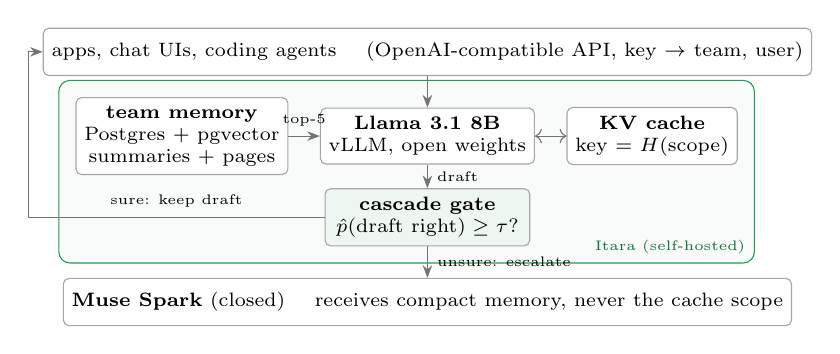
\begin{tikzpicture}[
  font=\scriptsize, node distance=3mm,
  box/.style={draw=black!35, rounded corners=2pt, fill=white, align=center, inner sep=3pt, minimum height=6mm},
  arr/.style={-{Stealth[length=1.6mm]}, draw=black!55},
]
\node[box, minimum width=7.4cm] (apps) {apps, chat UIs, coding agents \quad(OpenAI-compatible API, key $\to$ team, user)};
\node[box, below=4mm of apps, minimum width=2.6cm] (llama) {\textbf{Llama 3.1 8B}\\vLLM, open weights};
\node[box, left=4mm of llama, minimum width=2.1cm] (mem) {\textbf{team memory}\\Postgres + pgvector\\summaries + pages};
\node[box, right=4mm of llama, minimum width=2.1cm] (kv) {\textbf{KV cache}\\key = $H(\text{scope})$};
\node[box, below=3mm of llama, minimum width=2.6cm, fill=itarawash] (gate) {\textbf{cascade gate}\\$\hat p(\text{draft right}) \geq \tau$?};
\node[box, below=4mm of gate, minimum width=7.4cm] (muse) {\textbf{Muse Spark} (closed) \quad receives compact memory, never the cache scope};
\begin{scope}[on background layer]
\node[draw=itaragreen, fill=itarawash!40, rounded corners=4pt, fit=(mem)(llama)(kv)(gate), inner sep=6pt, label={[font=\tiny, text=itaragreen!70!black, anchor=south east]south east:Itara (self-hosted)}] {};
\end{scope}
\draw[arr] (apps) -- (llama);
\draw[arr] (mem) -- node[above, font=\tiny]{top-5} (llama);
\draw[arr, <->] (kv) -- (llama);
\draw[arr] (llama) -- node[right, font=\tiny]{draft} (gate);
\draw[arr] (gate) -- node[right, font=\tiny]{unsure: escalate} (muse);
\draw[arr] (gate.west) -| node[above, pos=0.25, font=\tiny]{sure: keep draft} ([xshift=-6mm]mem.south west) |- (apps.west);
\end{tikzpicture}}
\caption{Itara. The open model drafts every answer from the team's memory, reusing the team's cached prefill. The gate keeps confident drafts and escalates the rest to the closed model with compact memory. Row-level security and scope-keyed caching keep teams apart.}
\label{fig:arch}
\end{figure}

Itara is a single server (Figure~\ref{fig:arch}) that speaks the OpenAI chat-completions API, so a client adopts it by changing a base URL. It runs the open model on vLLM~\citep{kwon2023vllm}, stores memory in Postgres with pgvector~\citep{pgvector}, and reaches the closed model through the Meta Model API~\citep{metamodelapi}.

\paragraph{Identity and isolation.} Each API key maps to one team and one user, and only its hash is stored. Identity never comes from client headers. Every memory row carries a team and, optionally, an owner. Postgres row-level security~\citep{postgresrls}, forced even for the table owner, limits every query to rows of the caller's team that are either shared or owned by the caller. Personal memory is private by default; code, documents and decisions are shared with the team.

\paragraph{Shared memory.} A document is split on blank lines into pages of at most 2{,}000 characters. The open model compresses each page into a JSON summary, one fact per sentence (who did what, and when), plus keywords. If it fails twice, the page's opening text is stored instead. Summaries are embedded with BGE-small~\citep{xiao2023cpack}, and the raw pages are kept behind them. A page the team already holds is never compressed again, a changed file replaces its old version, and a source can be removed. A question retrieves its top $k{=}5$ summaries by reciprocal rank fusion~\citep{cormack2009rrf} of a cosine-similarity ranking and a full-text ranking:
\begin{equation}
\mathrm{score}(m)=\sum_{r\in\{\text{vec},\text{text}\}} \frac{1}{60+\mathrm{rank}_r(m)},
\end{equation}
with ties broken by id so that retrieval is deterministic. Code sources are labelled with their commit and conversation sources with their session date, which the compression prompt uses to resolve relative times.

\paragraph{Permission-scoped KV cache.} A request to the open model carries a cache salt $s=H(\text{team})$ if all the memory it retrieved is shared, or $H(\text{team}\,\|\,\text{user})$ if any of it is private. vLLM mixes the salt into the hash of the first KV block, so prefix hits only happen between requests with the same scope. A teammate asking about the same code reuses the prefill. A member of another team never hits the cache, even with an identical prompt, and so cannot learn anything from its timing~\citep{song2024earlybird}. The closed model receives memory but never the salt.

\paragraph{Routes and modes.} Each question takes one of three routes. On \emph{local\_memory} the open model answers with the top-5 summaries; on \emph{escalate\_compact} the closed model answers with the same summaries; on \emph{escalate\_raw} it answers with the raw pages behind them. The gateway runs in one of three modes. Accurate mode sends every question to the closed model with memory, fast mode lets the cascade gate below decide, and local mode never calls the closed model. Requests with tool calls, which is what coding agents send, skip the gate. They receive the team's memory as a system message and go on with their tools unchanged.

\paragraph{Gates.} The \emph{rule gate} is a baseline. It escalates questions longer than 200 tokens or containing a fenced code block. The \emph{per-route gate} fits, for each route, a logistic model of $P(\text{right}\mid x)$ on 18 features of the question, the retrieved memory and the open model's draft, and picks
\begin{equation}
\hat r(x)=\arg\max_{r} \; \hat P_r(\text{right}\mid x)-\lambda\,\widehat{\mathrm{cost}}_r(x),
\end{equation}
where the cost is estimated in dollars before the call. Sweeping $\lambda$ traces a cost--accuracy curve. Its training labels are each route's actual correctness on the item. The \emph{cascade gate}, which Itara ships, is simpler. The open model always drafts first, and a single logistic score $\hat p$ that the draft is right is computed from six confidence features:
\begin{itemize}
\item the mean and the minimum token log-probability of the draft;
\item the share of its tokens with probability below one half;
\item how well four resamples at temperature~1 agree with the draft, by cosine similarity and by exact first-line match;
\item the probability of ``yes'' when the model is asked whether its answer is correct and supported by the memory.
\end{itemize}
The resamples and the self-check reuse the draft's cached prefix, so they add little prefill. If $\hat p<\tau$ the question escalates, with summaries when most of the retrieved memory is code and with raw pages otherwise.

\paragraph{Accounting and the cap.} Every model call is recorded with the token counts the model reports, tagged with the request it belongs to. Before a paid call, its worst-case cost is reserved under a lock against a hard cap, so concurrent requests cannot overrun it, and the call's output is limited to what was reserved. An admin view shows the routes taken, cached tokens reused and spend per person and per team. The release includes a live dashboard and a command-line tool.

\section{Experimental setup}
\label{sec:setup}

\paragraph{Models and infrastructure.} The open model is Llama~3.1~8B Instruct~\citep{llama3}, served by vLLM with prefix caching on one H100 on Modal. The closed model is Muse Spark~1.2 through the Meta Model API~\citep{metamodelapi}. It is a reasoning model, so its output tokens include its reasoning, and we use its default effort unless stated. Answers are generated at temperature~0.

\paragraph{Benchmarks.} For code we use all 300 SWE-bench Lite issues~\citep{jimenez2024swebench}, posed as file localisation, a step recent agent pipelines rely on~\citep{xia2024agentless}. The model names at most five files to change, and an answer counts as right only if every file in the gold patch is among them, so no judge is needed. Each repository is a team, and its memory is the files in the BM25-retrieved context distributed with the benchmark (about 13K tokens per issue). For conversations we use 300 questions from LoCoMo~\citep{maharana2024locomo} (categories 1--4, sampled with a fixed seed). Each conversation is a team and each session a memory source. The closed model judges these answers at minimal effort~\citep{zheng2023judge}. We checked \handChecked{} randomly sampled verdicts by hand, across conditions, and agreed with the judge on \handAgree.

\paragraph{Conditions.} \emph{Muse, full context} sends the closed model all of the retrieved code (\directIn{} prompt tokens on average) or the whole conversation (\directInLoco). It is the accuracy reference and the denominator for every token share. The other conditions are \emph{always escalate} (with summaries or with raw pages), the \emph{rule gate}, \emph{Llama + memory} (never escalate) and Itara's \emph{cascade gate}. The \emph{oracle router} knows every route's correctness and picks the cheapest right one, so no gate choosing among these routes can beat it.

\paragraph{Metrics and protocol.} Accuracy is the share of items answered right. Cost is the closed model's tokens, prompt plus completion, as a share of the reference's on the same items; we also report the prompt-only share. Gates are trained and scored out of fold, with five folds grouped by team so that a repository or conversation never appears in both training and test. Intervals on accuracy gaps are paired bootstrap 95\% intervals over items, with 4{,}000 resamples~\citep{efron1993bootstrap}. The pass rule is applied to point estimates at each benchmark's 10\% operating point.

\paragraph{Team replay.} To measure sharing, we replay SWE-bench tasks on one repository with $n\in\{1,2,4,8,16\}$ simulated engineers doing two tasks each, either as one team (shared memory and cache) or each working alone. Tasks are ordered either by overlap with files the team has already touched (\emph{related}) or at random. Pages ingested per engineer measures the gateway's work independently of timing.

\section{Results}
\label{sec:results}

\begin{table*}[t]
\centering
\small
\caption{Main results. Gap: accuracy minus Muse with the full context, in points, with a paired bootstrap 95\% interval. Token share: Muse prompt + completion tokens relative to the reference on the same items; prompt share counts prompt tokens only. Kept: questions answered by the open model. On LoCoMo the rule gate never escalates (the questions are short and contain no code blocks), so it matches Llama + memory.}
\label{tab:main}
\begin{tabular}{lrcrrr}
\toprule
Condition & Accuracy (\%) & Gap (pts) [95\% CI] & Token share (\%) & Prompt share (\%) & Kept (\%)\\
\midrule
\rows{tab_main.tex}
\bottomrule
\end{tabular}
\end{table*}

\begin{figure*}[t]
\centering
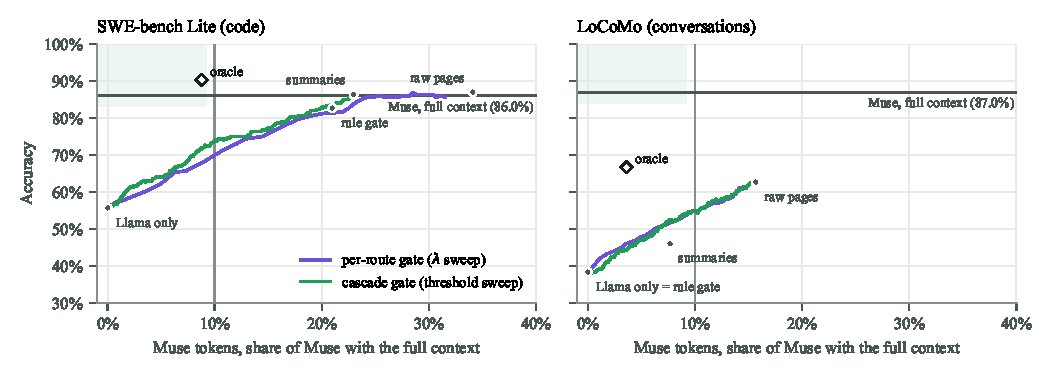
\includegraphics[width=\textwidth]{generated/fig_accuracy.pdf}
\caption{Accuracy against the closed model's tokens. Lines sweep each gate's threshold or $\lambda$ (out of fold). Dots are fixed routes; the diamond is the oracle router. The shaded box is the pre-registered pass region: within 3 points of the full-context reference at $\leq$10\% of its tokens.}
\label{fig:accuracy}
\end{figure*}

\subsection{On code, team memory keeps the closed model's accuracy}
\label{sec:memory}

Table~\ref{tab:main} and Figure~\ref{fig:accuracy} cover every condition. Sending every question to the closed model with the top-5 memory summaries scores \accSweCompact\%, against \accSweDirect\% with the full context (gap \gapSweCompact, interval \gapLoSweCompact{} to \gapHiSweCompact). We see no measurable loss. The closed model reads \inputSweCompact\% of the prompt tokens it would otherwise receive, \escInDefault{} instead of \directIn{} per question. Giving it the raw pages behind the summaries instead reaches \accSweRaw\% at \inputSweRaw\% of the prompt.

The total token share of the summary route is \shareSweCompact\%, though, not 9\%. Muse writes about \escOutDefault{} tokens of reasoning and answer per escalation, however short its prompt. With a reasoning model, compression removes the cost of the context but leaves the model's own output as a floor.

Muse has very likely seen these public repositories in training, which makes code localisation a lenient test of memory. The reference names the right files for \sweUnseenAcc\% of the \sweUnseenN{} issues whose gold file was not in its retrieved context at all. To measure what the memory itself adds, we ran two more baselines on the same issues after the main results. Given only the issue and no context, Muse localises \accQuestionOnly\% (\countQuestionOnly/300). Team memory adds \memoryOverQuestionOnly{} points to that (\countCompact/300, interval \memoryOverQuestionOnlyLo{} to \memoryOverQuestionOnlyHi) and is also cheaper, \$\usdMemory{} against \$\usdQuestionOnly{} per thousand questions, because Muse reasons for longer when it has no context. On a private codebase the model would know nothing in advance, and memory would be the only source. LoCoMo, where the answers exist only in the team's conversations, is the strict test (Section~\ref{sec:loco}).

The second baseline asks whether summaries beat plain retrieval. Searching the raw pages directly with the same hybrid search, with no summaries and nothing to build, scores \accPages\% (\countPages/300), against \accSweCompact\% for summaries (gap \memoryOverPages, interval \memoryOverPagesLo{} to \memoryOverPagesHi). Including the cost of building the memory for these 300 questions, the two cost about the same (\$\usdPagesDirect{} and \$\usdMemory{} per thousand). Per question, though, summaries send Muse a third of the prompt (\promptCompact{} tokens against \promptPages) and cut its bill by \museDropPages\%, so the build pays for itself after about \breakEvenPages{} questions on the same memory. Plain retrieval is a strong baseline at this scale. Summaries match its accuracy, cost less as a team keeps asking, and are what the open model reads in fast and local modes.

\subsection{The gate has a real signal but a hard budget}

\begin{table}[t]
\centering
\small
\caption{How well each signal separates the open model's right drafts from wrong ones (AUC, out of fold; 0.5 is chance).}
\label{tab:auc}
\begin{tabular}{lcc}
\toprule
Signal & Code & Conv.\\
\midrule
\rows{tab_auc.tex}
\bottomrule
\end{tabular}
\end{table}

\begin{table}[t]
\centering
\small
\setlength{\tabcolsep}{5pt}
\caption{Gates at each benchmark's 10\% budget (out of fold). Random: escalating the same share of tokens at random. The per-route gate uses 18 features and the cascade gate six confidence features. The last two rows are upper bounds.}
\label{tab:gate}
\begin{tabular}{lrrr}
\toprule
Gate & Acc. (\%) & Tokens (\%) & Random (\%)\\
\midrule
\rows{tab_gate.tex}
\bottomrule
\end{tabular}
\end{table}

The open model's confidence is informative (Table~\ref{tab:auc}). The strongest single feature is whether four resamples repeat the draft's answer, and mean token log-probability and the self-check also carry signal. All of them come from the open model alone, with no calls to the closed model. At the 10\% budget (Table~\ref{tab:gate}), the cascade gate scores \cascadeSwe\% on code against \randomSwe\% for random escalation with the same tokens, and keeps \cascadeKeptSwe\% of questions on the open model.

The per-route gate does worse at the budget (\perRouteSwe\%), despite a higher AUC for its draft score. It fits 18 features for each of three routes on about 480 training items per fold, and decides on the difference between two noisy probabilities. On conversations only \draftRightLoco\% of drafts are right, so a 10\% budget already escalates most questions and ranking them matters little.

Two upper bounds show why 10\% is out of reach for any gate that judges only the draft. A perfect draft check, which escalates exactly the wrong drafts, would score \perfectSwe\% on code but needs \perfectShareSwe\% of the tokens. The questions a good gate escalates are also the expensive ones: the closed model writes \escTokWrongSwe{} tokens on questions the open model got wrong, against \escTokRightSwe{} on those it got right. Only the oracle passes on code (\accSweOracle\% at \shareSweOracle\%), because it also knows when the closed model will fail.

\subsection{What a question costs}
\label{sec:cost}

\begin{table}[t]
\centering
\small
\setlength{\tabcolsep}{3pt}
\caption{The cost of 1{,}000 code questions, closed-model tokens and GPU time together, on the same 300 SWE-bench Lite issues; latency is per question. Prices: Muse's list prices, and an H100 at \$\hundredRate{} an hour charged as if each request had it alone, memory build included. Muse + raw pages: the pages behind the retrieved memories, without summaries. Random: as many escalations as the cascade at 10\%, mean of 1{,}000 draws. RouteLLM: an off-the-shelf router~\citep{ong2025routellm} deciding from the question alone. $^\dagger$Budget chosen after the run. $^\ddagger$Added after the results (Sections~\ref{sec:memory} and~\ref{sec:cost}). The live cascade's latency is measured end to end with six questions in flight; the two other $^\ddagger$ rows were answered eight at a time, so their latencies are not comparable with the rest.}
\label{tab:cost}
\begin{tabular}{lrrrr}
\toprule
Option & Acc.\,(\%) & \$/1k & \$/1k right & Median\,(s)\\
\midrule
\rows{tab_cost.tex}
\bottomrule
\end{tabular}
\end{table}

Token shares leave out two costs, the GPU that runs the open model and the time a user waits. Table~\ref{tab:cost} prices each option on the same 300 code questions from the saved answers, so this analysis calls no model. Muse is charged its exact tokens at list price. The GPU is charged at Modal's listed H100 rate for each request's open-model time, as if the request had the GPU to itself. That overstates it, since the deployment serves up to 32 requests at once. Every option that reads the memory also pays for building it: \buildMinutesSwe{} minutes of H100 time for these issues, or \$\buildUsdSwe{} per thousand questions, which a team asking more questions of the same code pays only once.

Team memory cuts the cost per question by \dropMemory\% at the same accuracy, and answers slightly sooner. The cascade cuts a further \dropCascadeMemory\% (\dropCascade\% in all). Its median answer arrives in \medCascade\,s instead of \medMemory\,s because most questions never leave the GPU, though at this budget it scores \cascadeSwe\% against \accSweCompact\%. Per correct answer it costs a little less than memory alone (\$\usdOkCascade{} against \$\usdOkMemory{} per thousand). At a 20\% budget it costs more than memory alone and is less accurate. Escalating the same number of questions at random is cheaper still but scores only \accRandomCount\%. The offline replay charges the cascade's confidence calls the draft's time again, since they were not timed.

So after the results we also ran fast mode live in the gateway, at the 10\% threshold, six questions at a time, timing each question end to end: draft, confidence calls and any escalation. It scores \accLive\% with a median wait of \liveMedian\,s (90th percentile \liveNinety\,s), escalating \liveEscalated\% of questions, at \$\liveUsd{} per thousand. The live gate re-runs the confidence probes, so it does not decide exactly as the replay does, but this is the number a deployment sees.

The simpler alternatives are close on code. Muse given raw pages, without summaries, costs \$\usdRaw{} per thousand for \accSweRaw\%. Once the closed model reasons for thousands of tokens per answer, shortening its prompt further saves little. The rule gate costs about the same as memory alone and is less accurate (\accSweRule\% against \accSweCompact\%).

\paragraph{Against an off-the-shelf router.} RouteLLM's BERT router~\citep{ong2025routellm}, trained on Chatbot Arena preferences and used as shipped, decides from the question alone whether the strong model is needed. We send the questions it picks straight to the closed model with team memory, and set its threshold to the most accurate one within each budget on these items, which favours it. Its score barely predicts when the open model's draft is wrong (AUC \aucRouterSwe{} on code and \aucRouterLoco{} on conversations, against the cascade's \aucCascadeSwe{} and \aucCascadeLoco). At the 10\% budget on code that difference is worth points: the cascade scores \accCascadeCost\% and the router \accRouterCost\%. The router is cheaper and faster, because it never drafts the questions it escalates. At 20\% the two are equally accurate (\accCascadeTwentyCost\% and \accRouterTwentyCost\%) and the router costs less, and on conversations at 10\% they are level (\accLocoCascadeCost\% and \accLocoRouter\%). The cascade's advantage is its signal, and that matters most when the budget is tight.

\paragraph{Sensitivity.} Two of the reference's answers reasoned up to the closed model's 262{,}144-token output limit and returned nothing. Dropping them from every option, team memory costs \$\usdMemoryNoRunaway{} per thousand against \$\usdDirectNoRunaway, \dropMemoryNoRunaway\% less rather than \dropMemory\%. Muse's API also bills cached prompt tokens at \$0.15 per million instead of \$1.25. On code it served \cachedShareSwe\% of the full-context prompts from its cache, since each issue's context differs, so nothing changes there. On conversations, where many questions share one transcript, \museCachedLoco\% was cached. Repriced at the cached rate, full context costs \$\usdLocoDirectCached{} per thousand against \$\usdLocoMemoryCached{} for team memory, and it is far more accurate on that benchmark.

Taken together, team memory justifies itself on cost alone. With an 8B open model, the cascade earns its extra complexity through latency and a lower bill, at some cost in accuracy, and it should earn more as the open model gets more questions right (Section~\ref{sec:bigger}).

\subsection{Sharing across a team}

\begin{figure}[t]
\centering
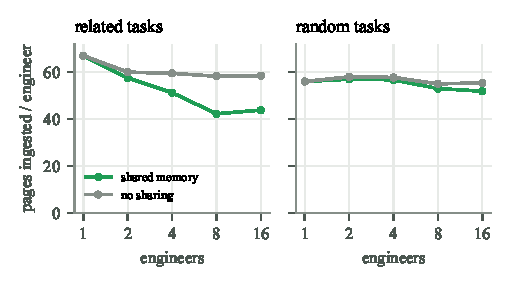
\includegraphics[width=\columnwidth]{generated/fig_scaling.pdf}
\caption{Pages ingested per engineer as the team grows (SWE-bench, one repository, two tasks per engineer).}
\label{fig:scaling}
\end{figure}

Figure~\ref{fig:scaling} shows each engineer's share of the work as the team grows. With shared memory, pages ingested per engineer fall by \dropSharedRelated\% at 16 engineers on related tasks, against \dropAloneRelated\% when each works alone. On random tasks the drop is \dropSharedRandom\% against \dropAloneRandom\%. The scoped KV cache behaved as designed on the H100 deployment. With one 6{,}150-token team memory, a teammate's request reused 6{,}144 cached prompt tokens and a request from another team reused none. On an H100 the wall-clock saving for 6K tokens is small (0.43\,s against 0.59\,s, mostly network round trips), so reused tokens are the better measure. The ingest saving is also small in dollars: at the measured build rate, ingest costs \$\teamIngestShared{} per engineer for two tasks with sharing and \$\teamIngestAlone{} alone, against about a cent of closed-model spend per question. At this scale sharing saves work and waiting more than money.

\subsection{On conversations, retrieval is the bottleneck}
\label{sec:loco}

On LoCoMo the best route, raw pages for every question, reaches \accLocoRaw\% at \shareLocoRaw\% of the tokens, against \accLocoDirect\% for the reference. Splitting the questions by whether retrieval found a memory from the session that holds the evidence (it did for \locoRetrieved\%) shows where the loss comes from. When retrieval found it, the closed model with raw pages scores \locoHitRaw\% against the reference's \locoHitDirect\%, while summaries alone score \locoHitCompact\%. Compression loses detail here, and the raw pages restore it. When retrieval missed, every gateway route scores \locoMissCompact--\locoMissRaw\%, while the reference, which reads everything, scores \locoMissDirect\%. The oracle router reaches only \accLocoOracle\%, so with this retrieval no routing policy can pass.

\subsection{The 10\% goal}
\label{sec:goal}

At 10\% of the closed model's tokens, the cascade gate reaches \cascadeSwe\% on code against \accSweDirect\% (gap \gapSweFull{} points, interval \gapLoSweFull{} to \gapHiSweFull), and \cascadeLoco\% on conversations against \accLocoDirect\%. Neither meets the pre-registered rule yet. On code the gate's upper bounds explain the gap, and on conversations retrieval does. Section~\ref{sec:discussion} discusses what would close it.

\section{Analyses chosen after the run}
\label{sec:posthoc}

The analyses in this section were chosen after we had seen the results. We report them with intervals and do not count any of them as meeting the goal.

\subsection{Larger budgets}

\begin{table}[t]
\centering
\small
\setlength{\tabcolsep}{4pt}
\caption{The most accurate option within each budget (any fixed route, either gate's sweep). $^\dagger$Budget chosen after seeing the results. \checkmark: within 3 points of the reference.}
\label{tab:budget}
\begin{tabular}{llll}
\toprule
Budget & Acc. (gap) & Option & Tokens (\%)\\
\midrule
\rows{tab_budget.tex}
\bottomrule
\end{tabular}
\end{table}

A team may prefer accuracy to the deepest saving. Table~\ref{tab:budget} adds 20\% and 25\% budgets as points on the curve. On code, sending every question with summaries matches the reference at \budgetQuarterShare\% of its tokens. The two runaway reference answers make up \runawayShare\% of its tokens, so we describe this as about a quarter. At that budget most of the saving comes from compact memory rather than from answering locally. Conversations stop at \locoCeiling\% whatever the budget.

\subsection{Lower reasoning effort}

\begin{table*}[t]
\centering
\small
\caption{Code, with the closed model at minimal reasoning effort (same memory, drafts and probes). Gaps against the full-context reference at the same effort (83.0\%) and at default effort (86.0\%), with paired bootstrap 95\% intervals. ``Other folds'': each fold's $\lambda$ is chosen on the other folds, removing in-sample selection.}
\label{tab:effort}
\begin{tabular}{lrcrcr}
\toprule
& & \multicolumn{2}{c}{vs.\ reference, same effort} & \multicolumn{2}{c}{vs.\ reference, default effort}\\
\cmidrule(lr){3-4}\cmidrule(lr){5-6}
Option & Acc. (\%) & Gap [95\% CI] & Tokens (\%) & Gap [95\% CI] & Tokens (\%)\\
\midrule
\rows{tab_effort.tex}
\bottomrule
\end{tabular}
\end{table*}

The closed model's output dominates the cost of an escalation, so we reran every closed-model condition at minimal reasoning effort on the same memory and drafts, with a full-context reference at the same effort (Table~\ref{tab:effort}). Output per escalation falls from \escOutDefault{} to \escOutMinimal{} tokens. On code the per-route gate then scores \minPerRoute\% against \minDirect\% (gap \minGap, interval \minLo{} to \minHi) at \minShare\% of the tokens, keeping \minKept\% of questions on the open model. Choosing $\lambda$ on the other folds gives a similar result, so in-sample selection does not explain it.

The point estimate falls inside the pass rule, but this is not a pass. The interval admits misses of over 5 points (the gap is at least $-3$ in \minP\% of resamples), the setting was chosen after the run, and the reference itself is weaker than at default effort. Against the default-effort reference the same gate misses by 5 points. Sending every question with summaries at minimal effort scores \minCompact\%, a gap of \minCompactGapDefault{} points to the \emph{default-effort} reference at \minCompactShareDefault\% of its tokens. Conversations do not move (\minLoco\%).

\subsection{Other open models}
\label{sec:bigger}

\begin{table*}[t]
\centering
\small
\caption{Each open model drafting the same questions, with the same team memory and closed-model answers (all but Llama~3.1~8B added after the run). Alone: the open model with team memory. 10\%: the cascade at a 10\% budget (its share of Muse's tokens). Perfect: escalating exactly the wrong drafts (share). AUC: the cascade's signal. Fast mode: Muse and GPU dollars per thousand questions, and the median wait. Llama~3.3~70B: FP8 on two H100s, code only. Muse Glimmer~30B: bf16 on one H100, reasoning strength low.}
\label{tab:open}
\begin{tabular}{lrrrrr}
\toprule
Open model & Alone (\%) & 10\% budget (\%) & Perfect check (\%) & AUC & Fast mode\\
\midrule
\rows{tab_open.tex}
\bottomrule
\end{tabular}
\end{table*}

To test whether the open model limits the gate, we swapped the drafting model and kept everything else fixed: the same questions, the same team memory (built by the 8B), the closed model's answers from the full run for every escalation, and the same out-of-fold gate training (Table~\ref{tab:open}).

\paragraph{Llama~3.3~70B.} On code, the 70B's drafts are right on \bigAlone\% of issues against \accSweLlama\% for the 8B (gain \gainAlone{} points, interval \gainAloneLo{} to \gainAloneHi). The cascade at 10\% scores \bigCascadeTen\% against \cascadeSwe\% (gain \gainCascade, interval \gainCascadeLo{} to \gainCascadeHi; better in \gainCascadeP\% of resamples), still \bigGapTen{} points from the reference. At a 20\% budget it scores \bigCascadeTwenty\% at \bigShareTwenty\% of the tokens, within \bigGapTwenty{} points of the reference, keeping \bigKeptTwenty\% of questions on the open model. A perfect draft check now passes: escalating exactly the \bigWrong\% of drafts that are wrong would score \bigPerfect\% at \bigPerfectShare\% of the tokens.

What remains is the gate. Its signal separates the 70B's right and wrong drafts less well than the 8B's (AUC \bigAuc{} against \aucCascadeSwe). Some of this is measurement noise. Re-drafting at temperature 0 under batching reproduced the 70B's answer for only \bigSame\% of items (\smallSame\% for the 8B), so its confidence features describe a slightly different draft from the one that was scored. The 70B also needs twice the GPU time per request.

\paragraph{A second opinion.} Two observations point to a better judge of the drafts. The self-check alone ranks the 70B's drafts better than the six-signal cascade (AUC \rawSelfBigAuc), and so does agreement between the two open models: when the 8B names the same first file as the 70B, the 70B is right far more often. Ranking drafts by the self-check, plus one when the 8B agrees, with no fitted weights, gives AUC \secondBigAuc{} and scores \secondBigTen\% at 10\% of the tokens (\secondBigTenNested\% with the threshold chosen on the other folds). That is \secondBigGain{} points over the cascade (interval \secondBigGainLo{} to \secondBigGainHi; better in \secondBigGainP\% of resamples), and \secondBigTwenty\% at 20\%. For the 8B's drafts, with the 70B as the second opinion, the gain is smaller (\secondSmallGain, interval \secondSmallGainLo{} to \secondSmallGainHi). We designed this rule after looking at these drafts, and it needs both open models running, so we treat it as the direction for the next gate rather than as a result.

Two other probes did not help. Running the self-check on the exact draft that was scored, rather than a fresh one, left its AUC unchanged (\bigExactSelfAuc{} against \rawSelfBigAuc), so re-drafting noise was not what limited it. A check that shows the model the issue and the memory's summaries of the file the draft names, and asks whether that file must change, was weaker (AUC \bigEvidenceAuc, and \smallEvidenceAuc{} for the 8B), and adding it to the self-check did not raise accuracy at 10\% (\bigSelfEvidenceTen\%). Fitting weights to a single signal does not help either. Pooled out-of-fold scores carry each fold's intercept, and since folds are whole repositories with different shares of right drafts, the fold rather than the signal decides much of the ranking (\texttt{eval/simple\_gate.py}).

\paragraph{Muse Glimmer 30B.} We then ran Meta's open-weight reasoning model, Muse Glimmer~30B (bf16, one H100), the same way on both benchmarks at its lowest reasoning strength. Two things change for the gate. vLLM returns probabilities for the reasoning as well as the answer, so the gate reads only the answer's tokens, and after reasoning those are nearly certain, so the probability features carry little. The self-check and the resamples both reason first. On code, Glimmer's drafts are right on \glimAlone\% of issues, \glimGainAlone{} points over the 8B (interval \glimGainAloneLo{} to \glimGainAloneHi). The cascade at 10\% scores \glimCascadeTen\% at \glimShareTen\% of the tokens and keeps \glimKeptTen\% of questions on the open model (\glimGainCascade{} over the 8B, interval \glimGainCascadeLo{} to \glimGainCascadeHi), still \glimGapTen{} points from the reference. A perfect judge of its drafts would pass (\glimPerfect\% at \glimPerfectShare\%). On conversations it adds nothing by itself (\glimLocoAlone\% against \accLocoLlama\%, gain \glimLocoGainAlone, interval \glimLocoGainAloneLo{} to \glimLocoGainAloneHi), as the retrieval analysis predicts.

Reasoning costs time. A Glimmer draft takes \glimDraftMed\,s at the median against \smallDraftMed\,s for the 8B. On our cost model, which charges each request a whole H100, fast mode with Glimmer costs \$\glimUsd{} per thousand code questions, against \$\usdCascade{} with the 8B and \$\usdMemory{} for sending every question to the closed model with memory. Glimmer's re-drafts reproduced the scored answer on \glimSame\% of code items. It is the best drafter we measured, and at this price it makes fast mode more accurate rather than cheaper.

\paragraph{Choosing the open model.} On code these runs suggest a simple rule. If every question goes to the closed model with memory, the open model only builds the memory. That is the most accurate setting we measured (\accSweCompact\% at \$\usdMemory{} per thousand questions, \medMemory\,s at the median), and the 8B is enough for it. For the cheapest and fastest answers, the 8B's cascade is the best of the three (\$\usdCascade, \medCascade\,s). Glimmer's cascade loses on all three counts to sending every question to the closed model with memory (\glimCascadeTen\%, \$\glimUsd{} and \glimMed\,s, against \accSweCompact\%, \$\usdMemory{} and \medMemory\,s), because each of its drafts and probes pays for reasoning on the GPU. Where nothing may leave the team's hardware, the open model answers alone, and there Glimmer is the clear choice (\glimAlone\% against \bigAlone\% and \accSweLlama\%); the release offers this as local mode. The 70B sits in between, and its cascade's gains over the 8B's are not yet distinguishable from chance. On conversations no open model helps much, since retrieval limits every route. In all three runs the memory was built by the 8B.

\section{Discussion}
\label{sec:discussion}

\paragraph{Where the cost goes.} We started from the premise that context dominates the bill. For a reasoning model that holds only until the context is compressed. After that, most of each escalation's cost is the closed model's own reasoning, so a 10\% budget allows only a few escalations and the gate has to be both accurate and selective. That leaves two levers: send fewer questions, with a better gate, or make each escalation cheaper, for instance with a lower reasoning effort, which moved code close to the bar in our post-hoc run.

\paragraph{What a gate can know.} The open model's confidence identifies its own wrong answers reasonably well. The oracle's extra advantage comes from knowing when the closed model will also fail, and no signal computed on the draft provides that. Routing studies that report only the cheap model's accuracy, or count calls instead of tokens, may understate this limit.

\paragraph{The path to the goal.} The 10\% goal remains Itara's target, and on code the measurements suggest it is reachable with more than nine days and one GPU. The pass region is not empty: the oracle router reaches \accSweOracle\% at \shareSweOracle\% of the tokens. The open model is what limits the gate. The 8B's draft is right on only \draftRightSwe\% of issues, so even a perfect draft check needs \perfectShareSwe\% of the tokens. With the 70B or Glimmer drafting, a perfect check passes, and the cascade at 10\% rises from \cascadeSwe\% to \bigCascadeTen\% and \glimCascadeTen\%. The gate's signal did not improve with the larger models, though, so the main lever now is a better judge of the drafts, such as the second opinion above, rather than a bigger model. The gates were also trained on only about 480 items per fold, and a deployed gateway collects more as a matter of course. On conversations a larger model is not enough, because retrieval caps every route, and better retrieval has to come first. These are expectations to test, not results.

\paragraph{Why open weights.} The shared cache needs control of the model's attention state, which closed APIs do not expose, and a cache is only reusable by the model that produced it. The layer that handles a team's repeated reading therefore has to be an open-weight model. We built and measured Itara with Llama and Muse Glimmer, but other open families would work as well.

\section{Limitations}
\begin{itemize}
\item \textbf{Simulated teams.} Teams are repositories and conversations, and the replay simulates engineers. We did not observe real teams.
\item \textbf{Models.} We used one closed model and three open models, two of them only after the run (Llama~3.3~70B on code, and Muse Glimmer~30B). Results may differ for others.
\item \textbf{An LLM judge} scores LoCoMo. The hand check agreed on \handAgree{} of \handChecked{} verdicts, and both disagreements were lenient calls by the judge.
\item \textbf{A lenient task.} File localisation on well-known repositories rewards prior knowledge; the reference is often right without seeing the file. It is also not patch generation, and we make no claim about repairing code.
\item \textbf{Pooled memory.} Each repository's memory holds the retrieved files of all its sampled issues, across versions, so a question can retrieve files the reference's prompt did not contain. We did not fix a snapshot per issue.
\item \textbf{Gate features and selection.} Confidence probes re-draft the answer, and re-drafting under batching does not always reproduce the scored draft. Thresholds come from out-of-fold sweeps on the same items, with no untouched test set. Pooling five folds' predictions under one threshold can blur the ranking, since folds are whole repositories with different intercepts; a deployed gate is a single model and does not have this problem. The live gate does not enforce a token ratio, and it was trained only on file paths and short conversational answers.
\item \textbf{Post-hoc choices} (budgets, reasoning effort, extra baselines, other open models) were made after seeing results. Choosing an operating point from a sweep on the same items is a mild selection, and our nested check suggests it is small here.
\item \textbf{Sample size.} With 300 items per benchmark, intervals on gaps are about $\pm$3 points. Item-level bootstrap intervals ignore clustering by repository and conversation.
\item \textbf{The cost model} is ours: list prices, and an H100 charged per request as if unshared. It counts no idle GPU time, startup, CPU or database. The offline cascade's confidence calls are estimated, not timed (the live run measures them). We compare against simpler retrieval and routing but not against an off-the-shelf prompt compressor~\citep{jiang2023llmlingua}.
\item \textbf{Cache scope.} We tested scope-keyed prefix caching on one server. Sharing the cache across servers (LMCache) was not evaluated.
\end{itemize}

\section{Conclusion}
Itara gives a team one open-weight model, one compressed memory and one permission-scoped KV cache, and calls a closed model only when the open model is unsure. On code, team memory lets the closed model match its full-context accuracy with under a tenth of the context, about a quarter of the tokens and roughly half the cost. The open model's confidence is a usable escalation signal, sharing memory makes each extra engineer cheaper, and the scoped cache keeps teams apart. On conversations, retrieval rather than routing limits accuracy. The goal we set in advance, matching the closed model at 10\% of its tokens, is not reached yet, but the measurements point the way. The oracle passes on code, the open model's accuracy is the main limit, and stronger open models lift the cascade at 10\% from \cascadeSwe\% to \bigCascadeTen\% (Llama~3.3~70B) and \glimCascadeTen\% (Muse Glimmer~30B). Next we plan a better judge of the drafts, gates trained on more questions, better retrieval and cheaper escalations. Every escalation also pairs the open model's draft with the closed model's answer on the team's own questions, which makes the gateway a natural source of data for improving the team's open model.

\section*{Reproducibility}
Code, per-item answers for every real-model run, gate replays and analysis notebooks are in the repository (\texttt{results/}). Every table and figure in this paper is generated from those files by \texttt{paper/generate.py}, which calls no model. Simulated runs used to test the pipeline are excluded from all reported numbers. After the main runs the gateway gained a few small changes (memory for tool requests, ingest that never compresses a page twice, an output limit per call); none of them affects a reported number.

\section*{Disclosure and use of AI assistance}
This work was carried out during the Meta Global AI Developer Hackathon (26 October--4 November 2026). The only earlier code in use, about 20 lines of a compression prompt from the author's earlier project, was imported in one marked commit; everything else was written during the event (see \texttt{DISCLOSURE.md}). AI coding assistants were used for research, planning, code and writing, and the author reviewed all design decisions, experiments and results. The benchmark data are public (SWE-bench Lite, LoCoMo), and no private or company data was used.

\bibliographystyle{plainnat}
\bibliography{references}

\end{document}
